\documentclass{cmn}

\tikzset{
  node/.style={
    draw,circle,inner sep=0.75mm,
  },
  tree/.style={
    level 1/.style={level distance=12mm,sibling distance=16mm},
    level 2/.style={level distance=12mm,sibling distance=8mm},
  }
}

\begin{document}
  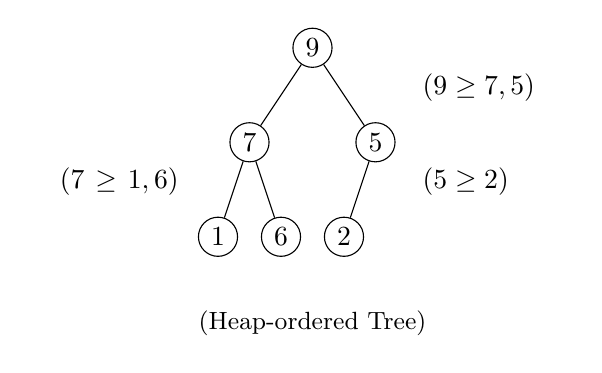
\begin{tikzpicture}[tree]
    \node[node] {9}
      child {
        node[node] {7}
        child {
          node[node] {1}
        }
        child {
          node[node] {6}
        }
      }
      child {
        node[node] {5}
        child {
          node[node] {2}
        }
        child { edge from parent[draw=none] }
      };

    \node[text width=18mm,align=left]  at ( 23mm,-5mm)  {($9 \geq 7, 5$)};
    \node[text width=18mm,align=right] at (-26mm,-17mm) {($7 \geq 1, 6$)};
    \node[text width=18mm,align=left]  at ( 23mm,-17mm) {($5 \geq 2$)};

    \node at (0,-35mm) {\small (Heap-ordered Tree)};
  \end{tikzpicture}
\end{document}
